\documentclass[11pt,a4paper]{article}
\usepackage[T1]{fontenc}
\usepackage[margin=2.3cm]{geometry}
\usepackage{amsmath,amssymb}
\usepackage{graphicx}
\usepackage[dvipsnames]{xcolor}
\usepackage{enumitem}
\usepackage[colorlinks=true,linkcolor=blue,urlcolor=blue]{hyperref}
\setlength{\parskip}{0.6em}
\setlength{\parindent}{0pt}
\begin{document}

\begin{center}{\LARGE\bfseries opensurrogate}\\[0.4em]{\large Replace a slow stiff chemistry solver by a fast neural stand-in, and audit it honestly.}\\[0.2em]\small PAN IIT OSS explainer \textbullet{} higher secondary to advanced undergraduate (levels 4-6)\end{center}

\section*{Why this exists}
Chemistry inside a flame is stiff and slow to simulate. This explainer shows how a small neural network can replace the chemistry solver for one time step, and, just as important, how to audit it: rollout error, mass conservation, speed-up and failure outside its training range.

\section*{The end goal}
Build a neural surrogate for stiff kinetics. The end goal is a neural surrogate for stiff kinetics, built from scratch in NumPy and audited against a trusted implicit solver. The same recipe applies to real combustion mechanisms and to any slow simulation you want to replace by a learned stand-in.

\section*{How the three sessions build up}
\begin{enumerate}[nosep]
\item \textbf{Session 1: A fast stand-in for a slow simulation} (Level 1, conceptual interactive model, 60 min).
\item \textbf{Session 2: A stiff chemical toy, an implicit solver and a fitted surrogate} (Level 2, mathematical engineering model, 80 min).
\item \textbf{Session 3: A neural surrogate and its honest audit} (Level 3, simulation and validation, 90 min).
\end{enumerate}

\section{Session 1: A fast stand-in for a slow simulation}

\subsection*{A. Real-world problem}
A combustion engineer wants the result of a chemical simulation for thousands of different conditions, but each run takes minutes. Running them all is too slow. The idea: run the slow simulation for a modest number of well-chosen conditions, learn the pattern 'conditions in, answer out', and let the learned pattern answer all the other conditions instantly. That learned pattern is called a surrogate. How many slow runs are enough, and how do we know the stand-in is good?

\subsection*{B. Concept and theory}
Our slow simulation follows a substance that decays at rate k (units 1/s): dy/dt = -k y, starting from y = 1, run for 1 second with 20000 tiny Euler steps. Its input is k (between 0 and 5) and its answer is the fraction left after 1 second, which is exp(-k) in exact mathematics. The surrogate is built from n training runs at evenly spaced values of k: for a new k it draws a straight line between the two nearest training runs (linear interpolation). Its error is the difference from the true answer. The worst-case error is the largest error over all k in the range. Using only the training runs and nothing else is the key limit: outside the range 0 to 5 the surrogate has no information.

\begin{itemize}[nosep]
\item k: decay rate, the input (1/s)
\item y: fraction of the substance left after 1 s, the answer (no unit (between 0 and 1))
\item n: number of training runs (no unit)
\item h: spacing between neighbouring training inputs, 5 / (n - 1) (1/s)
\item error: absolute difference between surrogate and true answer (no unit)
\end{itemize}

\begin{equation*}
\frac{dy}{dt}=-k\,y,\qquad y(0)=1\;\Rightarrow\;y(1\,\mathrm{s})=e^{-k}
\end{equation*}

\begin{equation*}
\hat y(k)=y_i+\frac{k-k_i}{k_{i+1}-k_i}\,(y_{i+1}-y_i),\qquad k_i\le k\le k_{i+1}
\end{equation*}

\begin{equation*}
\text{worst-case error}=\max_{0\le k\le 5}\left|\hat y(k)-e^{-k}\right|
\end{equation*}

\begin{center}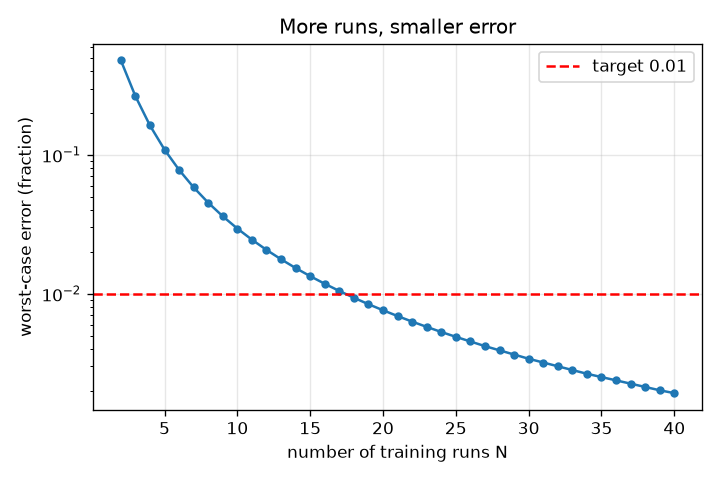
\includegraphics[width=0.85\linewidth]{figures/s01_error_vs_runs.png}\\\small Worst-case error against the number of training runs; 18 runs are the fewest that pass the 0.01 target.\end{center}

\subsection*{E. Worked example}
Build the surrogate from 6 runs (k = 0, 1, 2, 3, 4, 5). What does it answer at k = 2.5, what is the true answer, and what is the error?
\begin{enumerate}[nosep]
\item The nearest training runs are k = 2 and k = 3: exp(-2) = 0.1353 and exp(-3) = 0.0498.
\item k = 2.5 is exactly half way, so the surrogate answer is the average: (0.1353 + 0.0498) / 2 = 0.0926.
\item The true answer is exp(-2.5) = 0.0821.
\item Error = 0.0926 - 0.0821 = 0.0105 (a bit above 0.01, so 6 runs are not enough for a 0.01 target at every k).
\end{enumerate}
\textbf{Answer.} The surrogate says 0.0926, the truth is 0.0821, the error is 0.0105 (about 13 percent of the answer).

\subsection*{F. Questions}
\begin{enumerate}[nosep]
\item \textbf{Conceptual.} Why can a surrogate built from runs at k = 0 to 5 not be trusted at k = 6? What does it actually answer there?
\item \textbf{Numerical.} A surrogate is built from 3 runs (k = 0, 2.5, 5). Find its answer and its error at k = 1.25.
\item \textbf{Graph and simulation interpretation.} In the error graph, where is the error largest, and why? What happens to that peak when you add runs?
\item \textbf{Design and optimisation challenge.} Each slow run takes 2 minutes. Design: how many runs do you need for a worst-case error below 0.01, and below 0.001? What does the tighter target cost in time? What changes if there are two inputs on a grid with the same spacing?
\end{enumerate}

\section{Session 2: A stiff chemical toy, an implicit solver and a fitted surrogate}

\subsection*{A. Real-world problem}
Chemistry inside a flame is stiff: some reactions finish in microseconds while the interesting changes take seconds. A simulation that must follow the fastest reaction with its time step becomes very expensive, and a surrogate is attractive. But first we need a trustworthy solver to produce the training data. How do you build one, how do you know it is right, and how many training runs does a surrogate need to reach a target accuracy?

\subsection*{B. Concept and theory}
The toy is the Robertson problem (1966), a standard stiff test with three species A, B, C (mass fractions y1, y2, y3 that always add to 1): A turns into B slowly (k1 = 0.04 per second), two B can turn one into C (k3 = 3e7), and B plus C turn back into A plus B (k2 = 1e4). The fast and slow rate constants differ by a factor of 7.5e8 (almost nine orders of magnitude). The Jacobian J (matrix of derivatives of the right-hand side) has an eigenvalue of size around a few thousand per second, so an explicit method must keep its step h below 2 divided by that, while the slow physics needs steps of seconds. Backward Euler defines the new state by y\_new = y + h f(y\_new) and solves this equation with Newton iterations; it is stable for every h but only first-order accurate, so we combine runs with step h and h/2 (Richardson extrapolation) to get second order. We validate on a linear chain A -\textgreater{} B -\textgreater{} C with k1 = 1 and k2 = 1e4, which has an exact solution. The surrogate maps (initial fraction y1(0), slow rate k1, time t) to the state at time t: a polynomial in these three inputs (scaled to [-1, 1], with ln t) fitted by least squares to runs drawn with a seeded Latin hypercube. Species B is about 1e-5 and varies by decades, so we fit log10(y2); the third fraction follows from y3 = 1 - y1 - y2.

\begin{itemize}[nosep]
\item y1, y2, y3: mass fractions of A, B, C (no unit)
\item k1, k2, k3: rate constants (k1 slow and an input; k2, k3 fast) (1/s (fractions as units of concentration))
\item h: time step (s)
\item J: Jacobian, matrix of derivatives of f with respect to y (1/s)
\item t: time at which the state is wanted (0.1 to 40) (s)
\item d: total degree of the polynomial (no unit)
\item R: number of training runs (no unit)
\end{itemize}

\begin{equation*}
\dot y_1=-k_1y_1+k_2y_2y_3,\quad \dot y_2=k_1y_1-k_2y_2y_3-k_3y_2^2,\quad \dot y_3=k_3y_2^2
\end{equation*}

\begin{equation*}
y_{n+1}=y_n+h\,f(y_{n+1}),\qquad y^{(m+1)}=y^{(m)}-\left(I-hJ\right)^{-1}\left(y^{(m)}-y_n-hf(y^{(m)})\right)
\end{equation*}

\begin{equation*}
\dot y=-k\,y:\quad y_{n+1}=(1-kh)\,y_n\ \text{(explicit)},\qquad y_{n+1}=\frac{y_n}{1+kh}\ \text{(implicit)}
\end{equation*}

\begin{equation*}
y_{\text{Richardson}}=2\,y_{h/2}-y_h \quad (\text{first-order error cancels})
\end{equation*}

\begin{equation*}
\hat y=\Phi(x)\,c,\qquad c=\arg\min_c\|\Phi(x)c-y\|^2,\qquad x=(y_1(0),k_1,\ln t)
\end{equation*}

\begin{center}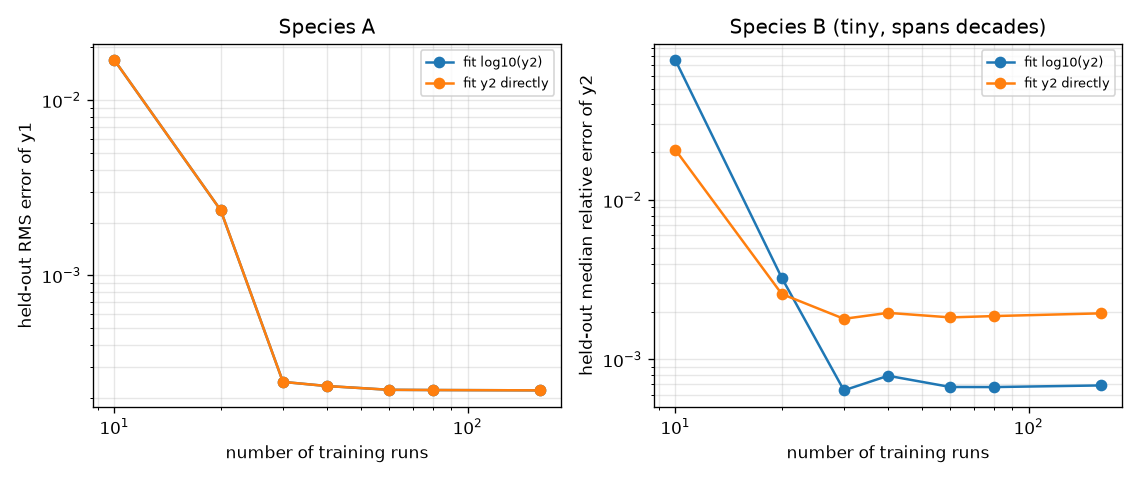
\includegraphics[width=0.85\linewidth]{figures/s02_error_vs_runs.png}\\\small Held-out error against the number of training runs, with and without log scaling of species B.\end{center}

\subsection*{E. Worked example}
For the fast step dy/dt = -10000 y with y(0) = 1 and a step h = 0.01 s, compute one explicit and one implicit Euler step by hand. Which one makes sense?
\begin{enumerate}[nosep]
\item k h = 10000 x 0.01 = 100.
\item Explicit: y1 = (1 - k h) y0 = (1 - 100) x 1 = -99. The solution should lie between 0 and 1 and decay: -99 is nonsense (unstable).
\item Implicit: y1 = y0 / (1 + k h) = 1 / 101 = 0.0099. It decays, as the exact solution exp(-100) does (about 0).
\item Rule of thumb: explicit needs k h below 2, here h below 2e-4 s; implicit works for any h.
\end{enumerate}
\textbf{Answer.} Explicit Euler gives -99 (unstable); implicit Euler gives 1/101 = 0.0099, which is stable and decays in the right direction.

\subsection*{F. Questions}
\begin{enumerate}[nosep]
\item \textbf{Conceptual.} Why is the explicit stability limit set by the fastest reaction even when we only care about the slow behaviour afterwards?
\item \textbf{Numerical.} For dy/dt = -2000 y and h = 0.002 s, compute k h, the explicit factor and the implicit factor. Is explicit Euler stable?
\item \textbf{Graph and simulation interpretation.} In the error graph, how does the held-out error change from 10 to 20 to 30 training runs, and why does it stop falling? Is the log fit always better?
\item \textbf{Design and optimisation challenge.} Design: you need the held-out RMS error of y1 below 0.003, and below 0.0005. How many runs (from 10, 20, 30, ...) do you need for each? What would you change if you needed 0.0001?
\end{enumerate}

\section{Session 3: A neural surrogate and its honest audit}

\subsection*{A. Real-world problem}
Inside a large combustion simulation the chemistry is solved again and again, in every grid cell, at every time step. A neural network that jumps the chemical state forward by one time step is a candidate stand-in. But a stand-in that is almost perfect for one step can be badly wrong after eighty, can create or destroy mass, and can fail without warning outside the conditions it was trained on. Before anyone trusts it, it must be audited against the true solver. How do you do that?

\subsection*{B. Concept and theory}
The surrogate predicts the state after one time step dt = 0.5 s of the Robertson problem. The state is coded as z = (y1, y3, s) with s = (log10(y2 + 1e-10) + 7) / 3 (log scaling for the tiny species B). The network is a residual map z\_next = z + 0.1 * net(z, k1) with two tanh hidden layers of 24 units. Backpropagation computes the gradient of the loss layer by layer with the chain rule (the derivative of tanh is 1 - h\textasciicircum{}2); Adam keeps running averages of the gradient and of its square and takes steps of size lr * m / (sqrt(v) + eps). A rollout feeds the network its own output; an error e in one step is carried into the next step, so errors accumulate. Training on several steps in a row (backpropagating through the unrolled steps) teaches the network to cope with its own errors. Conservation: a free network predicts y1, y3 and s independently, so y1 + y2 + y3 is not forced to stay 1. The conserved network predicts only y1 and s and computes y3 = 1 - y1 - y2, so the total is exactly 1. A hand-sized model shows why drift matters: if each step adds a relative error eps to a process that conserves mass, the total drifts by eps * (1 - q\textasciicircum{}n) / (1 - q) after n steps, with q the surrogate's per-step factor.

\begin{itemize}[nosep]
\item z: coded state seen by the network (no unit)
\item s: log-scaled species B (no unit)
\item dt: surrogate time step (0.5) (s)
\item n: number of rollout steps (80) (no unit)
\item eps: relative error of the surrogate step in the toy (no unit)
\item a, q: true and surrogate per-step factor in the toy (a = 0.95, q = a (1 + eps)) (no unit)
\item lr: Adam learning rate (no unit)
\end{itemize}

\begin{equation*}
z_{j+1}=z_j+0.1\,\mathrm{net}(z_j,k_1),\qquad s=\frac{\log_{10}(y_2+10^{-10})+7}{3}
\end{equation*}

\begin{equation*}
L=\sum_{u=1}^{K}\left\|\frac{z_u-z_u^{\mathrm{true}}}{0.1}\right\|^2\quad(K=1:\ \text{one-step},\ K>1:\ \text{multi-step})
\end{equation*}

\begin{equation*}
m\leftarrow\beta_1m+(1-\beta_1)g,\quad v\leftarrow\beta_2v+(1-\beta_2)g^2,\quad \theta\leftarrow\theta-\mathrm{lr}\,\frac{m/(1-\beta_1^t)}{\sqrt{v/(1-\beta_2^t)}+\epsilon}
\end{equation*}

\begin{equation*}
y_3=1-y_1-y_2\quad(\text{conserved output})
\end{equation*}

\begin{equation*}
\text{drift}_n=\epsilon\,\frac{1-q^{n}}{1-q},\qquad q=a(1+\epsilon)
\end{equation*}

\begin{center}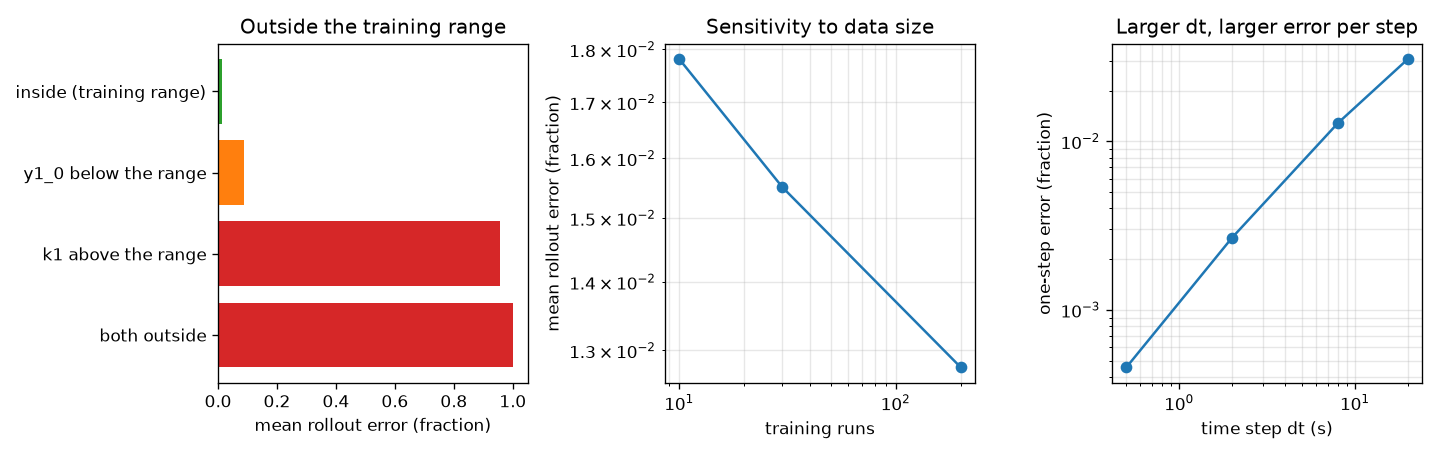
\includegraphics[width=0.85\linewidth]{figures/s03_audit.png}\\\small The audit: error outside the training range, sensitivity to data size, and one-step error against the time step.\end{center}

\subsection*{E. Worked example}
In the toy model (a = 0.95 per step, relative step error eps = 2 percent) compute the true A, the surrogate A and the total-mass drift after 50 steps, with a free output.
\begin{enumerate}[nosep]
\item True A = 0.95\textasciicircum{}50 = 0.0769.
\item Surrogate factor q = 0.95 x 1.02 = 0.969, so surrogate A = 0.969\textasciicircum{}50 = 0.2071 (almost three times too large).
\item Each step adds eps x A of mass, so drift = eps (1 - q\textasciicircum{}50) / (1 - q) = 0.02 x (1 - 0.2071) / 0.031 = 0.512.
\item The free network has created 51 percent more mass than exists; a conserved output computes B = 1 - A and has drift exactly 0.
\end{enumerate}
\textbf{Answer.} True A 0.0769, surrogate A 0.2071, drift 0.512 for the free output and 0 for the conserved output.

\subsection*{F. Questions}
\begin{enumerate}[nosep]
\item \textbf{Conceptual.} A surrogate has a one-step error of 0.0005 but a rollout error of 0.2 after 80 steps. How is that possible, and what two remedies does this session test?
\item \textbf{Numerical.} In the toy with a = 0.95 and eps = 1 percent, how much mass has been created after 100 steps with a free output? What if the output were conserved?
\item \textbf{Graph and simulation interpretation.} In the error figure, compare the one-step-trained and the 2-step-trained conserved networks. What do the curves say about error growth and about the mass drift of each?
\item \textbf{Design and optimisation challenge.} Design: you must deliver a surrogate with every held-out y1 error below 0.06 over 80 steps, mass drift below 1e-12, and a measured speed-up of at least 50 times over a one-at-a-time solver. Which options from this session do you choose, and which would you avoid? Justify with the numbers.
\end{enumerate}

\section{Real-world mini-project}
\textbf{Build and audit a surrogate for a stiff chain.} You are given the stiff three-species chain A -\textgreater{} B -\textgreater{} C with k1 = 1 per second and k2 = 1e4 per second (it has an exact solution, \texttt{chain\_exact} in Session 2). Build a one-step neural surrogate with your own data (use \texttt{chain\_rhs} and the backward Euler solver), roll it out, and audit it against the exact solution. Use the Session 3 network code: only the right-hand side and the data change.

\section{The path ahead}
\begin{enumerate}[nosep]
\item \textbf{Session 4: Know when you are outside.} An ensemble of five networks with a flag that raises an alarm for inputs outside the training range.
\item \textbf{Session 5: Tame the worst case.} A training recipe (more rollout steps, loss weights on the fast transient, a better loss for species B) aimed at the worst case.
\item \textbf{Session 6: One network for many time steps.} A network that takes dt as an extra input and works from dt = 0.5 s to 20 s.
\item \textbf{Session 7: Beat the vectorised solver.} A faster surrogate (smaller or batched in a smarter way) and a careful timing report.
\item \textbf{Session 8: Real hydrogen kinetics and element conservation.} The same pipeline for an 8-species hydrogen-oxygen mechanism, with a conservation-aware output layer for each element.
\end{enumerate}

\section{Answers and hints}

\subsection*{Session 1}
\begin{enumerate}[nosep]
\item \textbf{Conceptual.} Hint: Think about what information the training runs contain, and what np.interp does outside the table. Solution: The training runs say nothing about k above 5. A lookup table cannot invent information: np.interp just repeats the last value, so at k = 6 it answers 0.0067 (the value at k = 5) while the truth is 0.0025, more than twice as small. Nothing in the surrogate warns that it has left its range.
\item \textbf{Numerical.} Hint: k = 1.25 is half way between the first two runs; the answers there are 1 and exp(-2.5) = 0.0821. Solution: Surrogate = (1 + 0.0821) / 2 = 0.541. True exp(-1.25) = 0.2865. Error = 0.541 - 0.2865 = 0.255, nearly 90 percent of the true answer: three runs are far too few where the curve bends.
\item \textbf{Graph and simulation interpretation.} Hint: Compare the bend of exp(-k) near k = 0 and near k = 5. Solution: The error peaks near k = 0 where exp(-k) bends most (its second derivative is largest there); a straight line between two runs cannot follow a bend. Adding runs makes the straight pieces shorter, so the peak shrinks; with 18 runs it is 0.0094, below the 0.01 line.
\item \textbf{Design and optimisation challenge.} Hint: Use runs\_needed in the lesson, then multiply by the cost per run. For two inputs a grid needs n times n runs. Solution: runs\_needed gives 18 runs for 0.01 (36 minutes) and 56 runs for 0.001 (112 minutes): ten times less error costs about three times more runs. With two inputs on a grid of 18 values each you need 18 x 18 = 324 runs (648 minutes) and with three inputs 5832. Trade-off: connect-the-dots wastes runs when there are several inputs, which is why Sessions 2 and 3 use fitted formulas and networks.
\end{enumerate}

\subsection*{Session 2}
\begin{enumerate}[nosep]
\item \textbf{Conceptual.} Hint: Think about what happens to a tiny error in the fast species at each step. Solution: An explicit step multiplies a small error in the fast mode by (1 - k h). If k h is above 2 that factor has size above 1, so the error grows at every step and wrecks the whole solution, even though the fast species itself has long finished changing. The implicit factor 1/(1 + k h) is below 1 for every h, so the step can follow the slow physics.
\item \textbf{Numerical.} Hint: k h = 2000 x 0.002; stable means the factor has size below 1. Solution: k h = 4. Explicit factor 1 - 4 = -3 (size 3, unstable: it flips sign and triples each step). Implicit factor 1 / (1 + 4) = 0.2 (stable). The limit for explicit is k h below 2, i.e. h below 0.001 s.
\item \textbf{Graph and simulation interpretation.} Hint: Compare the printed numbers from lesson.py; think about the number of polynomial terms (84) and the polynomial's own limit. Solution: The held-out RMS error of y1 is 0.0169 with 10 runs, 0.0024 with 20 and 0.00025 with 30, then stays near 0.0002 up to 160 runs: with few runs the fit has more terms than information, and later the error is the limit of a degree-6 polynomial, not of the data. The log fit is not always better: with 10 runs the direct fit of y2 has a smaller relative error (0.021 against 0.076); from 30 runs on, the log fit wins, by a factor of about 2 to 3 at 160 runs (0.0007 against 0.0019).
\item \textbf{Design and optimisation challenge.} Hint: Use runs\_for\_target(0.003) and runs\_for\_target(0.0005). Solution: 20 runs reach 0.003 and 30 runs reach 0.0005. Half as many extra runs again (30 instead of 20) buys a ten times smaller error, but more runs cannot go below the plateau near 0.0002: for 0.0001 you must change the model (a higher polynomial degree or a different surrogate) rather than add runs. Assumptions: the same input ranges and a random Latin hypercube with seed 7; a different seed can move these numbers a little.
\end{enumerate}

\subsection*{Session 3}
\begin{enumerate}[nosep]
\item \textbf{Conceptual.} Hint: Where do the inputs of step 2 come from? Solution: The one-step error is measured from the TRUE state. In a rollout the network's own, slightly wrong output becomes the input of the next step, a state it never saw in training, so its error is bigger there and the errors compound. Remedy 1: train on several steps in a row (multi-step training), which reduces the step-80 error from 0.22 to 0.009. Remedy 2: for mass, build the conservation into the output layer (y3 = 1 - y1 - y2), which removes the drift exactly.
\item \textbf{Numerical.} Hint: drift = eps (1 - q\textasciicircum{}n) / (1 - q) with q = 0.95 x 1.01. Solution: q = 0.9595, q\textasciicircum{}100 = 0.0156, so drift = 0.01 x (1 - 0.0156) / 0.0405 = 0.243: 24 percent extra mass. With a conserved output the drift is exactly 0. Sanity check: eps = 2 percent gives 0.617, so the drift is roughly proportional to eps.
\item \textbf{Graph and simulation interpretation.} Hint: Read the values at step 80 from lesson.py: the y1/y3 error and the mass drift. Solution: The one-step-trained rollout error grows from 0.004 at step 1 to 0.22 at step 80; the 2-step-trained one is 0.0035 at step 1 and 0.009 at step 80, flat after step 10. Both conserved networks have mass drift 1e-16 (zero up to rounding), while the free one-step network has drifted by 0.28 and the free 2-step network by 0.02: multi-step training lowers the drift but only the structure removes it.
\item \textbf{Design and optimisation challenge.} Hint: Use the conserved/free, one-step/multi-step comparison, the speed test and the extrapolation test. Solution: Choose a conserved output with 2-step training: its worst y1 error over 100 held-out runs is 0.056, its mass drift is 1e-16 and it is more than 50 times faster than the solver run one at a time (hundreds of times in our timings). Avoid one-step training (error 0.22) and a free output (drift 0.28). Trade-offs: the speed-up against a vectorised solver is only a few times; and the guarantee is only for inputs inside the training range, where the error is 0.012; outside (k1 above the range) it is 0.96, so the deliverable needs a stated validity range.
\end{enumerate}

\section{How to join}
Read \texttt{CONTRIBUTING.md} in the repository, then pick an issue labelled \texttt{good first issue}. Repository: \url{https://github.com/KrunalPanchal1995/opensurrogate}

\end{document}
